\subsubsection{Voo Pairado (Hover)}

Neste cenário de voo pairado, o objetivo é que o drone suba até uma altura determinada e permaneça nessa altura até o fim da simulação. Além de analisar o desempenho do controlador de altitude, é interessante observar o comportamento dos controladores de posição nos eixos \(X\) e \(Y\), além dos controladores de arfagem, guinada e rolagem.

Parâmetros da simulação: \\

- Tempo total: 25 segundos;\\
- Altura desejada: 2 metros; \\
- Posição em \(X\) e \(Y\): 0.

1) Coordenada Z

\begin{figure}[H]
	\centering
	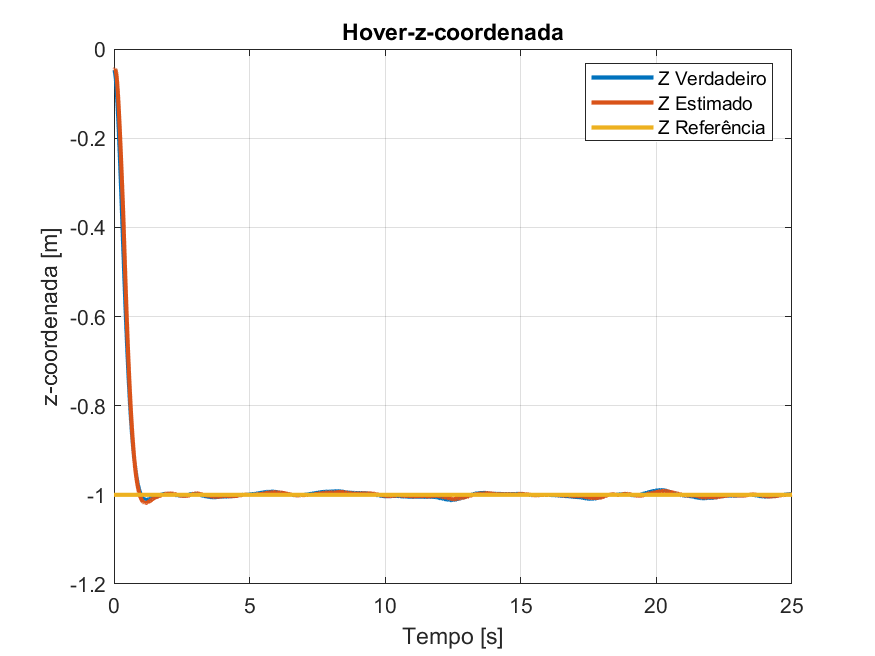
\includegraphics[width=1\textwidth]{Hover-z-coordenada.png}
	\caption{Coordenada Z para o Cenário de Voo Pairado}
	\label{fig:hover-z-coordenada}
\end{figure}

Analisando o gráfico, podemos observar que o tempo de estabilização é rápido, por volta dos 3 segundos, após o qual o sistema atinge a estabilidade próximo ao valor de referência. Um pequeno overshoot é visível no início, mas é bem controlado, e o erro em regime permanente é mínimo, indicando um bom desempenho do controlador para manter a altitude.

2) Coordenadas X e Y

Abaixo estão os gráficos das coordenadas \(X\) e \(Y\) do quadricóptero ao longo do tempo:

\begin{figure}[htbp]
    \centering
    \subfloat[Coordenada X para o Cenário de Voo Pairado]{
        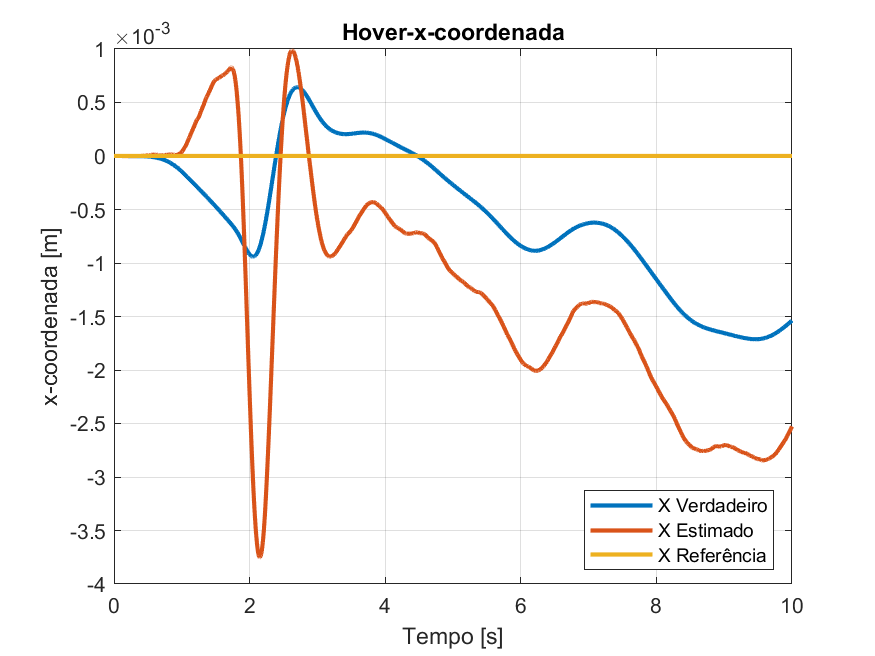
\includegraphics[width=0.45\textwidth]{Hover-x-coordenada.png}
        \label{fig:hover-x-coordenada}
    }
    \hfill
    \subfloat[Coordenada Y para o Cenário de Voo Pairado]{
        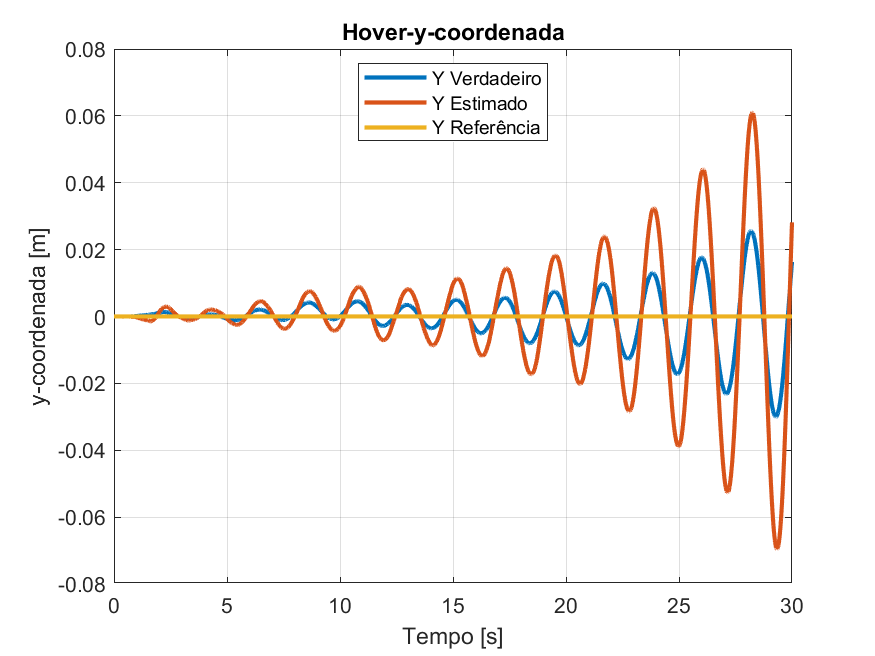
\includegraphics[width=0.45\textwidth]{Hover-y-coordenada.png}
        \label{fig:hover-y-coordenada}
    }
    \caption{Coordenadas X e Y para o Cenário de Voo Pairado}
    \label{fig:hover-x-y-coordenadas}
\end{figure}

No dois gráficos, podemos observar oscilações crescentes em torno do valor de referência com o tempo. No gráfico do eixo \(Y\), vemos que o valor verdadeiro aumenta ao longo do tempo proporcionalmente com os valores estimados, na curva de \(X\), apesar das altas oscilações dos valores estimados, o valor verdadeiro consegue se manter próximo ao valor de referência.

%Para ambos os eixos, uma possível solução é ajustar os ganhos \(K_p\) e \(K_d\) para suavizar a resposta e aumentar o amortecimento, além de adicionar um ganho integral \(K_i\) para reduzir o erro em regime permanente.

3) Ângulos de Rolagem, Arfagem e Guinada

A seguir estão os gráficos para os ângulos de rotação do quadricóptero: rolamento (roll), arfagem (pitch) e guinada (yaw).

\begin{figure}[htbp]
    \centering
    \subfloat[Arfagem para o Cenário de Voo Pairado]{
        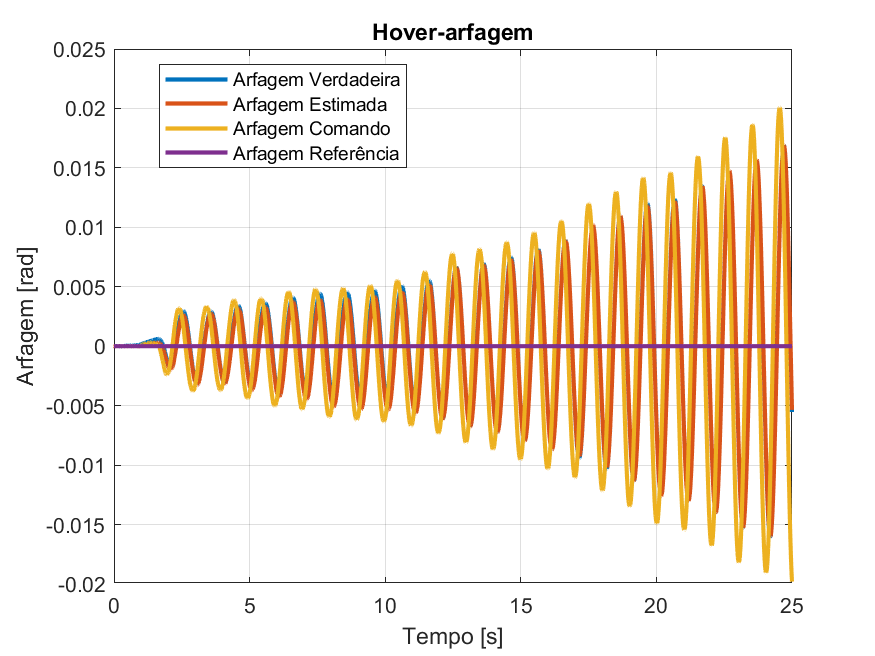
\includegraphics[width=0.45\textwidth]{Hover-arfagem.png}
        \label{fig:hover-arfagem}
    }
    \hfill
    \subfloat[Guinada para o Cenário de Voo Pairado]{
        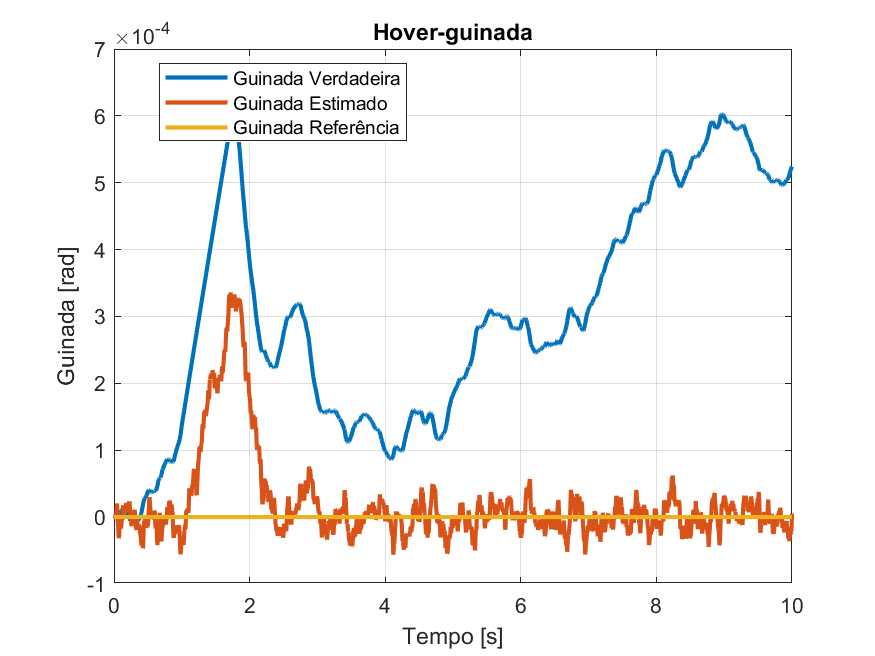
\includegraphics[width=0.45\textwidth]{Hover-guinada.png}
        \label{fig:hover-guinada}
    }
    \caption{Arfagem e Guinada para o Cenário de Voo Pairado}
    \label{fig:hover-arfagem-guinada}
\end{figure}

\begin{figure}[H]
	\centering
	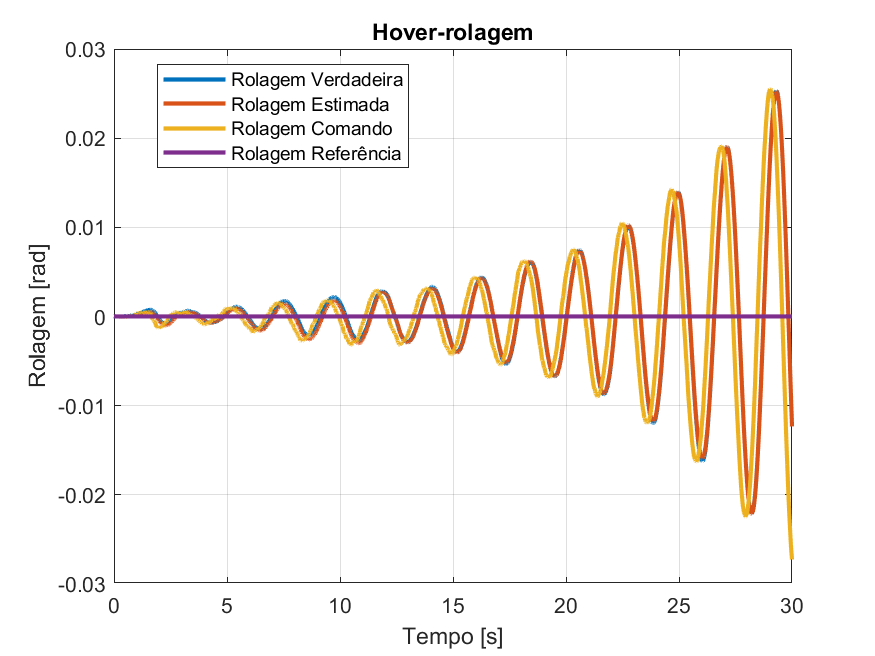
\includegraphics[width=0.5\textwidth]{Hover-rolagem.png}
	\caption{Rolagem para o Cenário de Voo Pairado}
	\label{fig:hover-rolagem}
\end{figure}

Nos gráficos, vemos que os ângulos de arfagem e rolamento apresentam oscilações crescentes ao longo do tempo, o que inclusive concorda com o comportamento que observamos nos eixos  \(X\) e  \(Y\) ,enquanto o ângulo de guinada permanece relativamente estável. Essas oscilações indicam uma possível falta de amortecimento no controlador, especialmente nos eixos de arfagem e rolamento.

Sendo assim, uma boa estratégia para iniciarmos nossas melhorias seria ajustar os parâmetros dos controladores de arfagem e rolagem, bem como os contralores da posição \(X\) e \(Y\).



%Para melhorar o desempenho, recomenda-se ajustar os parâmetros do controlador para reduzir as oscilações nesses eixos, aplicando amortecimento adicional e revisando os ganhos de controle. Isso deve resultar em um sistema mais estável e menos propenso a oscilações crescentes.

%Conclusão Geral para o Cenário de Voo Pairado

%No cenário de voo pairado, o controlador de altitude apresenta um bom desempenho, mas os controladores de posição e atitude nos eixos \(X\) e \(Y\), assim como os controladores de rotação (roll e pitch), mostram sinais de instabilidade. Ajustes nos parâmetros de controle são recomendados para melhorar a resposta geral e a estabilidade do sistema, especialmente em situações que exigem controle preciso de posição e orientação.




%---------------------------------------------------------------------
% INDICE REMISSIVO
%---------------------------------------------------------------------
\phantompart
\printindex
%---------------------------------------------------------------------
